% ======================================================================
% THESIS DRAFT -- edit this file for metadata, prose and chapter order.
% Compile from thesis_report/ with XeLaTeX (latexmk -xelatex main.tex).
% Overleaf: upload this folder, select main.tex, choose XeLaTeX.
% Formatting: preamble.tex | References: references.bib | Help: README.md
% All chapter text stays here so sections are easy to exchange with an AI.
% ======================================================================
\documentclass[11pt,a4paper,oneside,openany]{memoir}
% Formatting lives here; edit thesis prose and metadata in main.tex.
% Based on the supplied supplements/example.tex and its unchanged KU package.
\usepackage{fontspec}
\usepackage{libertine}
\usepackage[english]{babel}
\usepackage{amsmath}
\usepackage{booktabs}
\usepackage{tabularx}
\usepackage{float} % Keep each compact result table beside its explanation.
\usepackage{microtype}
\usepackage{xcolor}
\usepackage{graphicx}
\usepackage{xurl} % Permit long source URLs to wrap in the bibliography.
\usepackage{pdflscape}
\usepackage{csquotes}
\usepackage[backend=biber,style=authoryear,sorting=nyt,maxcitenames=2]{biblatex}
\addbibresource{references.bib}
\setcounter{biburllcpenalty}{7000}
\setcounter{biburlucpenalty}{8000}
\setcounter{biburlnumpenalty}{7000}

% Find the original KU package and its logos without moving or changing them.
\makeatletter
\def\input@path{{supplements/}}
\makeatother
\graphicspath{{figures/}{supplements/}}
\usepackage[english,samf,hyperref]{ku-frontpage}
% The template requests a semibold series absent from this font setup.
% Select bold explicitly instead of relying on repeated font substitutions.
\renewcommand{\KUsemibold}{\bfseries}
\pdfstringdefDisableCommands{\def\\{ }}

% Memoir controls the body layout; the KU package controls the cover.
\setlrmarginsandblock{30mm}{30mm}{*}
\setulmarginsandblock{28mm}{28mm}{*}
\checkandfixthelayout
\OnehalfSpacing
\chapterstyle{hangnum}
\pagestyle{plain}
\setcounter{secnumdepth}{2}
\setcounter{tocdepth}{1}
\setlength{\emergencystretch}{2em}

% Memoir can prevent the template from patching some title commands.
% These fallbacks support both patched and unpatched versions of memoir.
\providecommand{\frontpageauthor}[1]{}
\providecommand{\frontpagetitle}[1]{}
\providecommand{\frontpagesubtitle}[1]{}
\providecommand{\frontpagedate}[1]{}

% Visible writing prompts can be hidden using \draftnotesfalse in main.tex.
\newif\ifdraftnotes
\draftnotestrue
\newcommand{\draftnote}[1]{%
  \ifdraftnotes
    \par\smallskip
    {\small\noindent\textcolor{KU}{\textbf{Draft task:} #1}\par}%
    \smallskip
  \fi
}


% ---- EDIT: cover details -----------------------------------------------
% Working title: revise freely. Keep it short to fit the example's cover.
\newcommand{\ThesisTitle}{Urban Accessibility\\and Airbnb Prices}
\newcommand{\ThesisSubtitle}{Euclidean and walking measures across three Nordic capitals}
\newcommand{\ThesisAuthor}{Ahmad Jibril Hemdi}
\newcommand{\ThesisDate}{Submission date to be confirmed}
\newcommand{\ThesisAdvisors}{Supervisors: Sandro Sousa \& Jason Burton}

\assignment{Master's thesis}
\author{\ThesisAuthor}
\title{\ThesisTitle}
\subtitle{\ThesisSubtitle}
\date{\ThesisDate}
\advisor{\ThesisAdvisors}
\frontpageauthor{\ThesisAuthor}
\frontpagetitle{\ThesisTitle}
\frontpagesubtitle{\ThesisSubtitle}
\frontpagedate{\ThesisDate}
% Optional cover illustration, placed in figures/:
% \frontpageimage{cover.png}
\kupdfsetup{\ThesisTitle}{MSc Social Data Science}{\ThesisAuthor}

% ---- EDIT: writing mode -----------------------------------------------
\draftnotestrue % Change to \draftnotesfalse to hide visible writing prompts.
% Hiding prompts does not mean the draft is complete; search for them first.

\begin{document}
\frontmatter
\begingroup
  \SingleSpacing
  \maketitle
\endgroup

% ======================================================================
% FRONT MATTER -- write the abstract after the results and conclusion.
% ======================================================================
\chapter*{Abstract}
\addcontentsline{toc}{chapter}{Abstract}
\draftnote{Write the final abstract last: problem, three-city data, matched
measurements, geographic evaluation, main qualified findings and contribution.
Report asking prices and observational evidence. Add verified numbers only.}

% Add acknowledgements or required declarations here after checking the
% programme's requirements. The example's PhD statement is not used.

\cleardoublepage
\tableofcontents
% Uncomment once actual figures/tables have been inserted:
% \listoffigures
% \listoftables

\mainmatter
% ======================================================================
% CHAPTER 1 -- INTRODUCTION
% Purpose: establish the problem, the gap, the questions and the contribution.
% Authority: ../docs/design/scientific_proposal.md (not a literature review).
% ======================================================================
\chapter{Introduction}
\label{ch:introduction}

\section{Motivation and research problem}
\label{sec:motivation}
This thesis examines how straight-line and walking-network representations of
urban accessibility relate to Airbnb nightly asking prices in
Copenhagen--Frederiksberg, Oslo and Stockholm. It compares what the two
representations measure, the information they add to price prediction,
geographic variation within cities, and transfer between cities.

\draftnote{Explain why accessibility measurement matters for the research
problem. Define asking price early. Support the motivation with literature
you have read and verified; distinguish listings from bookings or revenue.}

\section{Research gap and contribution}
\label{sec:gap}
\draftnote{Build one argument from the literature to the gap: representation,
geographic evaluation and transfer. State the contribution of their combined
comparison without claiming universal novelty or a causal effect.}

\section{Research questions}
\label{sec:research-questions}
The analysis is organized around four research questions:
\begin{enumerate}
  \item[RQ1.] How do matched Euclidean and walking accessibility measurements
  differ across the three cities?
  \item[RQ2.] What information do these measurements add to within-city price
  prediction, and what complementary adjusted associations are observed?
  \item[RQ3.] How do predictive performance and accessibility contributions
  vary across geographic validation designs and held-out neighbourhoods?
  \item[RQ4.] How do relative-price predictions and accessibility contributions
  transfer across the six source--target city directions?
\end{enumerate}

\section{Scope and thesis roadmap}
\label{sec:roadmap}
The study uses June 2026 Inside Airbnb listings for conventional entire
dwellings. Its evidence is observational. Chapter~\ref{ch:literature} reviews
related literature, and Chapter~\ref{ch:theory} develops the theoretical
framework. Chapter~\ref{ch:data} describes the data and study areas, and
Chapter~\ref{ch:methods} defines measurement and evaluation.
Chapter~\ref{ch:results} presents the evidence in research-question order,
followed by discussion in Chapter~\ref{ch:discussion} and conclusions in
Chapter~\ref{ch:conclusion}.

% ======================================================================
% CHAPTER 2 -- RELATED LITERATURE
% Purpose: review prior evidence and establish the research gap.
% Add only checked sources to references.bib; use \textcite / \parencite.
% ======================================================================
\chapter{Related Literature}
\label{ch:literature}
\label{sec:related-literature}
\draftnote{Synthesize verified studies around their data, accessibility
measures, pricing outcomes and evaluation designs. Explain how they inform
the research gap; avoid claiming universal novelty. Cite only sources that
have been read and checked.}

\section{Accessibility and Airbnb pricing}
\label{sec:recent-airbnb-literature}
\draftnote{Review recent relevant Airbnb studies of accessibility or asking
prices. Identify their findings, contexts and limitations, and distinguish
asking prices from transactions, bookings and revenue.}

\section{Euclidean accessibility in Airbnb research}
\label{sec:representations-literature}
\draftnote{Review Airbnb studies that measure proximity or opportunities with
straight-line distance. Describe the destinations, distance definitions and
pricing outcomes, and explain what this representation captures and misses.}

\section{Walking accessibility in Airbnb research}
\label{sec:walking-literature}
\draftnote{Review Airbnb studies using pedestrian-network distances, travel
times or reachable opportunities. Compare their inputs and assumptions with
Euclidean approaches without assuming that network measures predict better.}

\section{Geographic generalization in Airbnb price prediction}
\label{sec:generalization-literature}
\draftnote{Review Airbnb price-prediction studies that evaluate geographic
generalization, including spatial holdouts or transfer where available.
Distinguish these from random validation and identify any evidence gap; do not
invent a study if a direct precedent cannot be verified.}

% ======================================================================
% CHAPTER 3 -- THEORETICAL FRAMEWORK
% Purpose: develop the concepts that motivate the analytical comparison.
% ======================================================================
\chapter{Theoretical Framework}
\label{ch:theory}
\label{sec:theoretical-framework}
\section{Hedonic pricing theory}
\label{sec:hedonic-pricing}
\draftnote{Explain hedonic pricing as a framework for relating prices to
property and location attributes. Connect it to Airbnb asking prices and
conditional associations without treating estimated coefficients as causal.}

\subsection{Spatial extensions of hedonic pricing}
\label{sec:spatial-hedonic-pricing}
\draftnote{Explain the spatial context of hedonic prices, including location,
spatial dependence and the limits of interpreting correlated attributes.
Relate this framework to the study's controls and geographic evaluation.}

\section{Accessibility concepts and representations}
\label{sec:accessibility-concept}
\draftnote{Define accessibility, proximity and reachable opportunities.
Explain Euclidean and walking representations and plausible relationships to
asking prices, including confounding and selection. Link the framework to
RQ1--RQ4 without assuming that measurement detail improves prediction.}

\section{Theoretical synthesis and analytical expectations}
\label{sec:expectations}
\draftnote{Connect the literature and theoretical framework to RQ1--RQ4.
Label expectations as conceptual; do not retrospectively call observed patterns
preregistered hypotheses. Avoid repeating the introduction.}

% ======================================================================
% CHAPTER 4 -- STUDY AREAS AND DATA
% Purpose: explain what is observed and which populations the results cover.
% Sources: ../docs/analysis/data_dictionary.md, source_registry.md,
% sample_audit.json, context_audit.json; ../outputs/tables/sample_flow.md.
% ======================================================================
\chapter{Study Areas and Data}
\label{ch:data}

The analysis combines Airbnb listing records, mapped destinations and pedestrian
networks, and official population statistics for Copenhagen--Frederiksberg,
Oslo and Stockholm. This chapter defines the populations represented by the
samples, the spatial units used to organise them, and the main qualifications
of the resulting measurements.

\section{Study areas and validation geography}
\label{sec:study-areas}
Copenhagen denotes the combined Copenhagen and Frederiksberg study area
throughout. Oslo and Stockholm use their accepted city study masks. These
three capital-city samples provide separate settings for comparing accessibility
representations and testing geographic prediction; they are not a representative
sample of cities.

Three spatial definitions serve different purposes. Accepted study masks
determine which listings are included. Inside Airbnb neighbourhood polygons
define operational validation groups: 11 in Copenhagen, 17 in Oslo and 11 in
Stockholm. Copenhagen combines ten districts with Frederiksberg; Oslo retains
Sentrum and Marka alongside its fifteen boroughs. Stockholm's fourteen provider
labels are mapped to eleven fixed groups. These are documented analytical
assignments, rather than certification that provider polygons reproduce current
official boundaries. Official native statistical areas separately provide the
denominators for population density.

Figure~\ref{fig:study-areas} shows the validation geography. Source coordinates
are handled in EPSG:4326; metric operations use EPSG:25832 in Copenhagen,
EPSG:25833 in Oslo and EPSG:3006 in Stockholm. The map's surrounding municipalities
are display context and do not determine sample membership.

% Manuscript map is rerendered from frozen SQL geometry; provenance and hashes
% are recorded in tables/data_assets_manifest.json. Original public map is preserved.
\begin{landscape}
\begin{figure}[p]
  \centering
  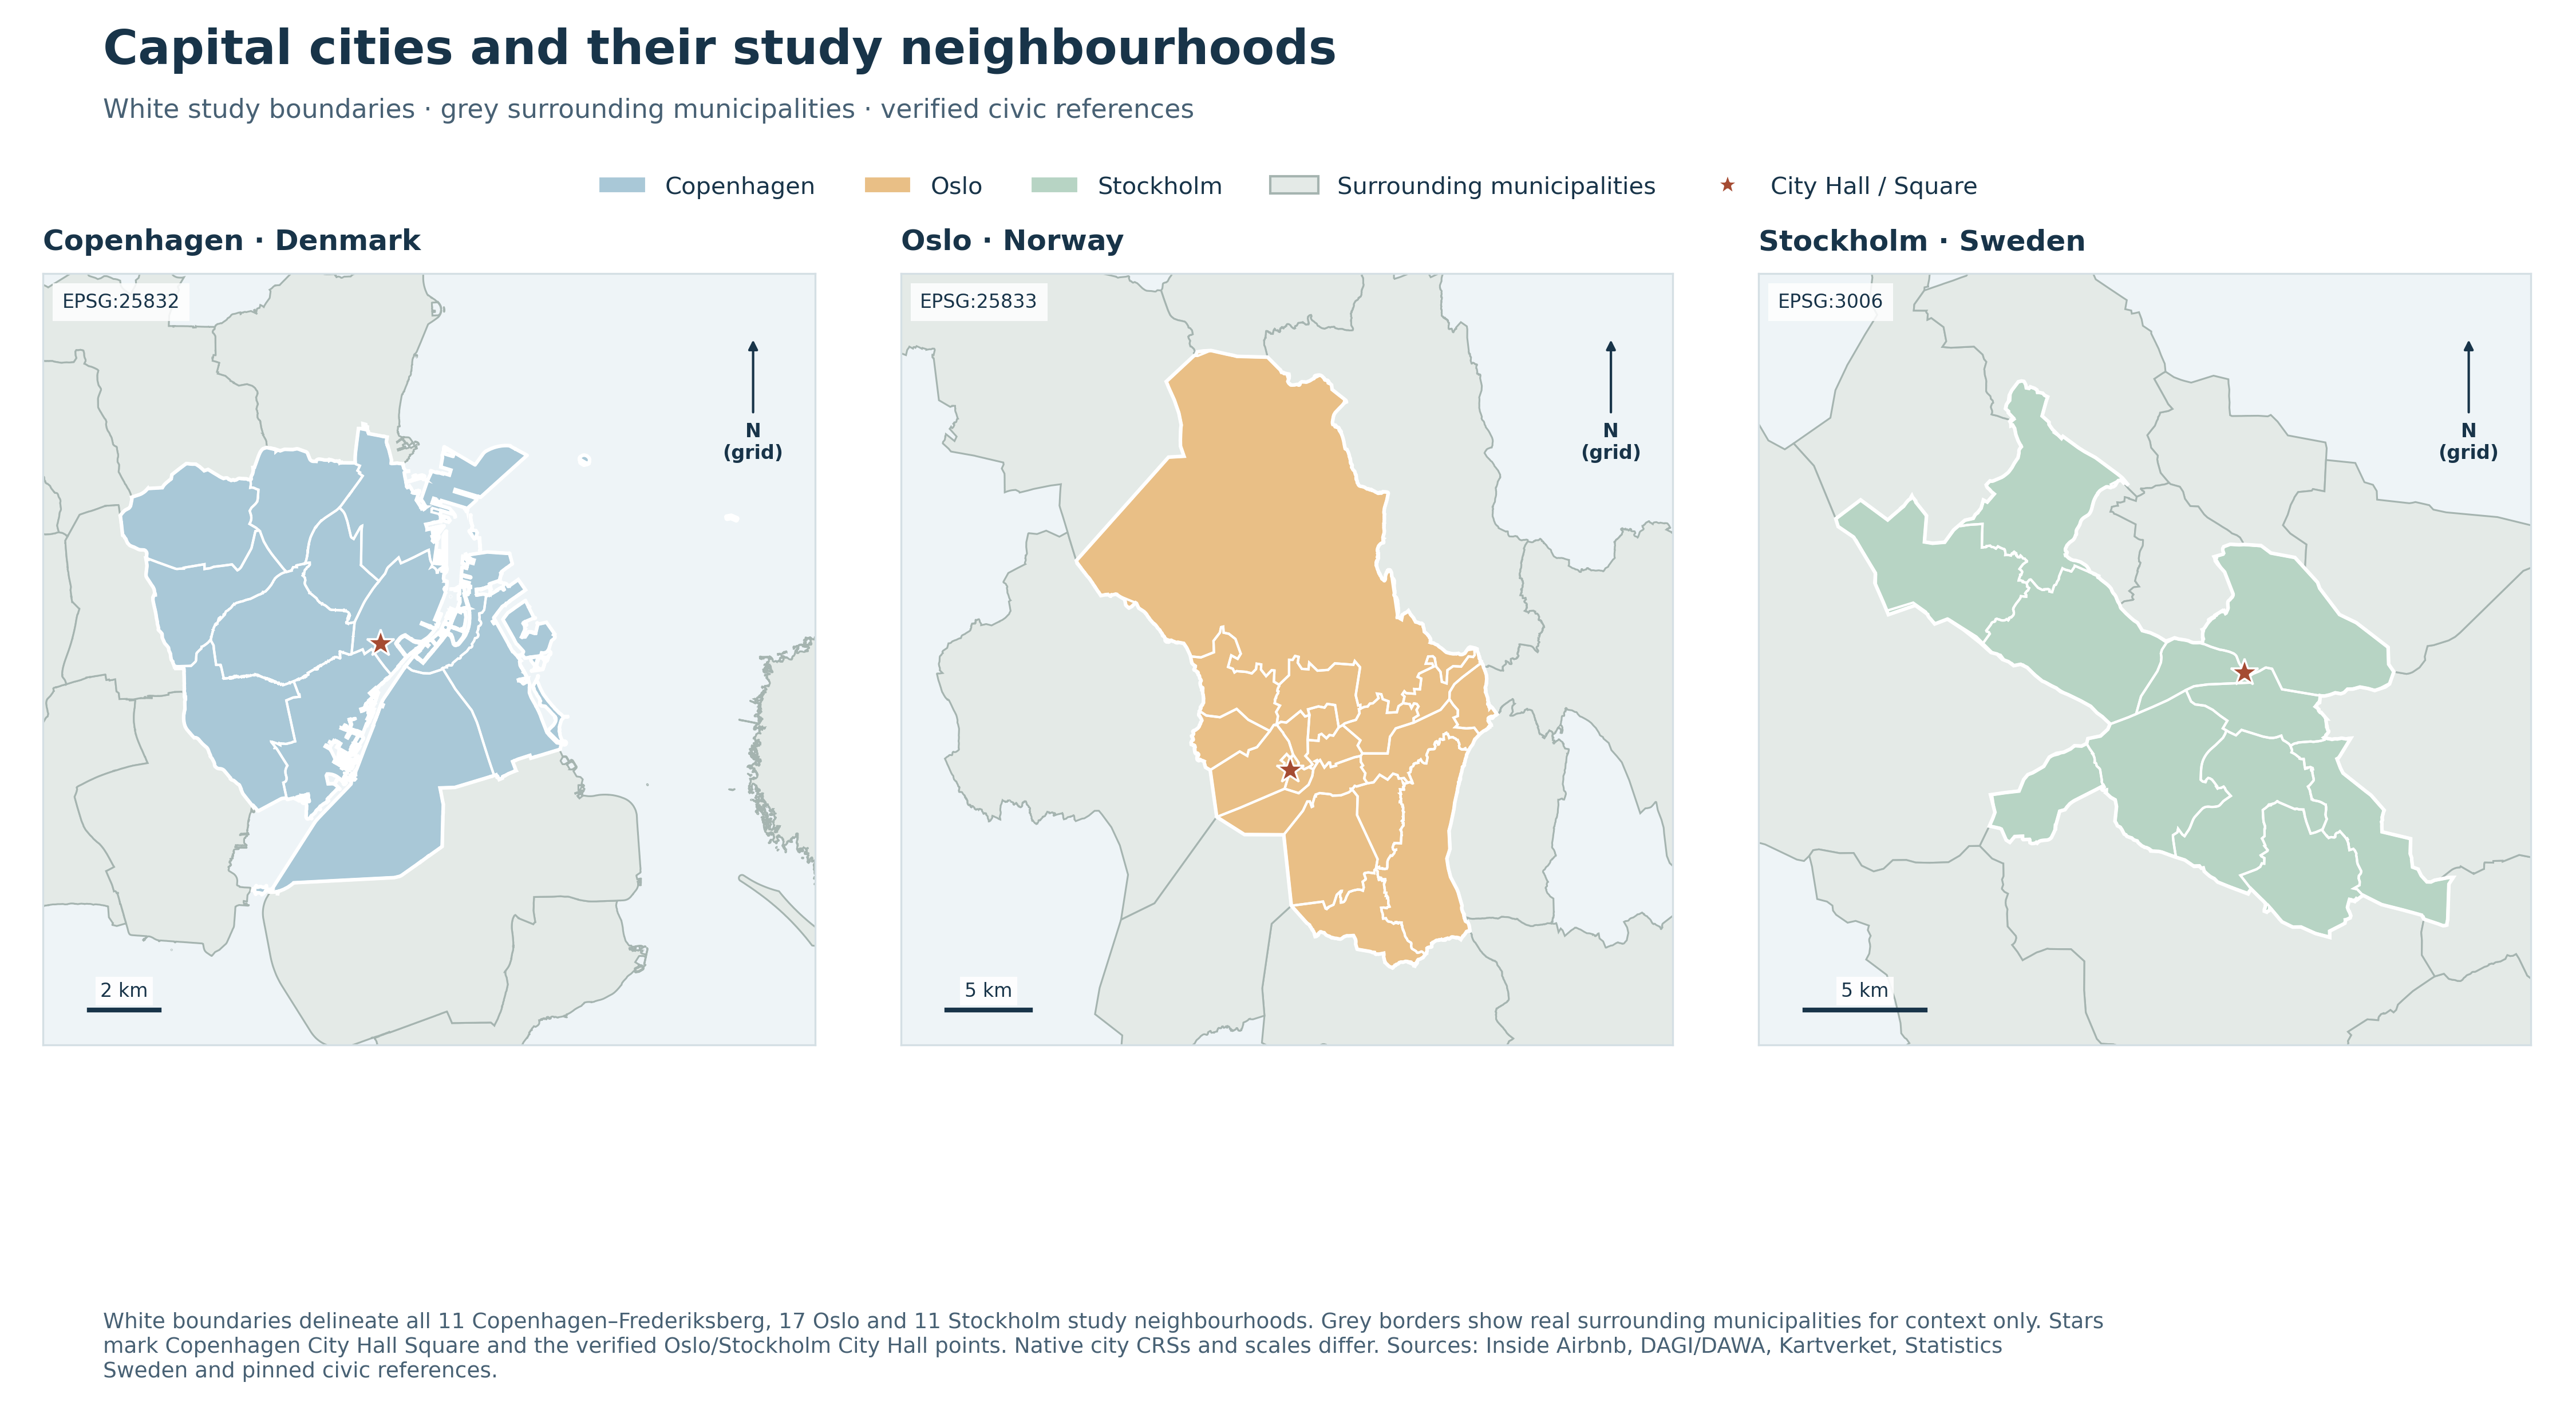
\includegraphics[width=\linewidth]{study_areas.png}
  \caption{Operational validation groups (white): 11 Copenhagen--Frederiksberg,
  17 Oslo and 11 Stockholm groups. Grey borders are October 2026 municipal
  context, not analytical June geography. Stars mark Copenhagen City Hall Square
  and Oslo/Stockholm City Halls; Copenhagen's analytical anchor is the City Hall
  building. Panels use the indicated CRSs, grid-north arrows and different scales.
  Sources: Inside Airbnb, DAGI/DAWA, Kartverket, Statistics Sweden and verified
  civic references.}
  \label{fig:study-areas}
\end{figure}
\end{landscape}

\section{Data sources and spatial coverage}
\label{sec:sources}
The listing sources are Inside Airbnb's detailed city datasets in the catalogue
batch dated 30 June 2026
\parencite{data_inside_cph2026,data_inside_oslo2026,data_inside_stockholm2026}.
This is a common snapshot designation, not evidence that every listing was
observed at the same instant. The records describe advertised accommodation.
Inside Airbnb notes that listing coordinates are displaced and that a snapshot
can include listings subsequently removed from the platform
\parencite{data_inside_assumptions}. Coordinates therefore support approximate
spatial measurement, rather than identification of exact properties.

% Generated by scripts/build_thesis_data_assets.py; do not edit values.
\begin{table}[H]
\centering\small
\caption{Principal analytical sources and reference periods.}
\label{tab:data-sources}
\begin{tabularx}{\textwidth}{@{}>{\raggedright\arraybackslash}p{0.23\textwidth}>{\raggedright\arraybackslash}X >{\raggedright\arraybackslash}p{0.25\textwidth}@{}}
\toprule
Input & Reference period and coverage & Analytical role \\
\midrule
Inside Airbnb & 30 June 2026 catalogue batch; city-specific listings and neighbourhood polygons & Asking prices, listing controls and validation groups \\
OpenStreetMap & 30 June 2026, 23:59:59 UTC; study extent with a 2 km extraction buffer & Pedestrian routes, destinations and civic anchors \\
Copenhagen / Frederiksberg population & 2026Q3; KKBEF1 / FOLK1A with native district or municipal areas & Population density \\
Oslo population & 1 January 2026; BEF001 with native areas for 17 units & Population density \\
Stockholm population & 31 December 2025 population; 31 December 2024 published land-plus-water areas & Population density \\
\bottomrule
\end{tabularx}
\par\smallskip
\begin{minipage}{\textwidth}\footnotesize
Sources: \parencite{data_inside_cph2026,data_inside_oslo2026,data_inside_stockholm2026,data_osm_license,data_kkbef1,data_folk1a,data_oslo_bef001,data_stockholm_yearbook}. Reference periods describe the data, not download dates. Copenhagen's population reference is 1 July 2026. Area definitions and source vintages differ across cities.
\end{minipage}
\end{table}


OpenStreetMap supplies the pedestrian graph, rail and bus destinations,
food/social and culture/tourism opportunities, and civic anchors. Analytical
extracts use a common historical timestamp of 30 June 2026 at 23:59:59 UTC and
a 2 km buffer around the study extent. The extracts were acquired later;
reference time and acquisition time are recorded separately. Destination
coverage and network connectivity remain source limitations. A finite zero
opportunity count is retained as zero, while unavailable routing or source
support remains missing. Chapter~\ref{ch:methods} defines the matched measures.

The source register records URLs, acquisition dates, geographic extents,
CRSs, licences and checksums. Raw bytes are retained unchanged, and
PostgreSQL/PostGIS holds the persistent analytical tables. The accompanying
provenance register documents source-specific qualifications and variable
definitions.

\section{Sample selection and missing data}
\label{sec:samples}
Eligibility is restricted to listings classified as entire homes/apartments in
six conventional dwelling types: rental units, condominiums, houses, lofts,
townhouses and villas. Shared and private rooms are excluded. Each retained
listing must have an original observed positive nightly asking price, fall
inside the accepted study mask, and have unique operational geography and
qualified context. Missing or nonpositive prices are excluded; quote prices
are not substituted.

% Generated by scripts/build_thesis_data_assets.py; do not edit values.
\begin{table}[H]
\centering\small
\caption{Listing selection and analytical samples.}
\label{tab:data-samples}
\begin{tabular}{lrrr}
\toprule
Stage & Copenhagen & Oslo & Stockholm \\
\midrule
Raw listings & 23,144 & 13,391 & 4,806 \\
Eligible entire dwellings & 21,080 & 11,776 & 3,834 \\
Observed positive asking price & 12,521 & 8,557 & 2,510 \\
Inside study area / price reference & 12,508 & 8,557 & 2,510 \\
Common predictive sample & 12,408 & 8,529 & 2,495 \\
Complete-case association sample & 12,285 & 8,152 & 2,348 \\
\addlinespace
Predictor missingness (\%) & 0.99 & 4.42 & 5.89 \\
Validation neighbourhoods & 11 & 17 & 11 \\
\bottomrule
\end{tabular}
\par\smallskip
\begin{minipage}{\textwidth}\footnotesize
Source: frozen study sample-flow and city-summary exports from Inside Airbnb listings. Selection is sequential through the predictive sample; association complete cases are a subset. Predictor missingness is the share of predictive rows missing at least one required predictor. All four predictive models share rows and folds; no missing outcome is imputed.
\end{minipage}
\end{table}


Table~\ref{tab:data-samples} distinguishes the inside-mask price-reference
population from the common predictive sample. Accessibility support removes
100, 28 and 15 further listings in Copenhagen, Oslo and Stockholm, respectively.
Every predictive specification uses the resulting common rows and folds,
including the control model. The substantial earlier price-related attrition
limits the population to which the findings apply; its causes are not inferred
from the retained records.

Table~\ref{tab:data-missingness} shows missing asking-price counts and percentages
before sample selection, including rooms. Its denominators differ from the
predictive samples.

% Generated by scripts/build_thesis_data_assets.py; do not edit values.
\begin{table}[H]
\centering\small\setlength{\tabcolsep}{4pt}
\caption{Missing asking prices by accommodation type before sample selection.}
\label{tab:data-missingness}
\begin{tabular}{@{}lrrrrrrrrr@{}}
\toprule
 & \multicolumn{3}{c}{Copenhagen} & \multicolumn{3}{c}{Oslo} & \multicolumn{3}{c}{Stockholm} \\ Accommodation type & $N$ & Missing & \% & $N$ & Missing & \% & $N$ & Missing & \% \\
\midrule
Entire rental unit & 13,588 & 5,260 & 38.7 & 8,100 & 2,157 & 26.6 & 2,622 & 893 & 34.1 \\
Entire condo & 5,599 & 2,617 & 46.7 & 2,546 & 804 & 31.6 & 355 & 177 & 49.9 \\
Entire home & 1,260 & 427 & 33.9 & 871 & 182 & 20.9 & 586 & 156 & 26.6 \\
Entire loft & 104 & 45 & 43.3 & 101 & 31 & 30.7 & 41 & 17 & 41.5 \\
Entire townhouse & 343 & 143 & 41.7 & 103 & 32 & 31.1 & 80 & 33 & 41.2 \\
Entire villa & 186 & 67 & 36.0 & 55 & 13 & 23.6 & 150 & 48 & 32.0 \\
Other entire property types & 288 & 30 & 10.4 & 153 & 21 & 13.7 & 147 & 23 & 15.6 \\
Private room & 1,756 & 694 & 39.5 & 1,398 & 305 & 21.8 & 794 & 190 & 23.9 \\
Shared room & 20 & 1 & 5.0 & 64 & 5 & 7.8 & 28 & 2 & 7.1 \\
Hotel room & 0 & 0 & -- & 0 & 0 & -- & 3 & 3 & 100.0 \\
\midrule
All original listings & 23,144 & 9,284 & 40.1 & 13,391 & 3,550 & 26.5 & 4,806 & 1,542 & 32.1 \\
\bottomrule
\end{tabular}
\par\smallskip
\begin{minipage}{\textwidth}\footnotesize
Source: original Inside Airbnb ingestions. $N$ is the listing count; Missing counts blank asking prices. Percentages are $100\times\mathrm{Missing}/N$ within city/type; a dash means $N=0$. Nonpositive prices are not missing. Room rows use source room type; other entire property types are pooled. Counts precede all sample filters.
\end{minipage}
\end{table}


Required-predictor missingness mainly concerns bedrooms: 123 values in
Copenhagen, 376 in Oslo and 147 in Stockholm; Oslo also has one missing
minimum-night value. Predictive preprocessing learns its replacements from
training data only. Association inference instead uses genuine complete cases.
The uniform eligibility limit for that analysis was raised from 5\% to 10\%
on 13 October 2026 after Stockholm's 5.8918\% missingness was observed. This
amendment permits the complete-case analysis without filling bedrooms or
outcomes, and does not remove selection into the observed sample.

\section{Asking prices and control variables}
\label{sec:variables}
The within-city outcome is the natural logarithm of the original observed
positive nightly asking price in DKK, NOK or SEK. It represents an advertised
price, rather than a completed booking or host revenue. Cross-city transfer
subtracts each city's frozen mean log price from its eligible inside-mask
reference population before accessibility filtering
(Section~\ref{sec:transfer-method}). This preserves a separate distinction
between native-currency asking prices and benchmarked relative prices.

Common controls describe accommodation capacity, bedrooms, bathrooms, property
type and minimum nights; Superhost status and host listing counts; and eight
amenities: Wi-Fi, dishwasher, washer, dryer, workspace, free parking, private
balcony and self check-in. Minimum nights and host listing counts use
$\log(1+x)$. Bathrooms follow the audited structured-field/text-parser rule.
Location controls are log population density and straight-line distance in
kilometres to a frozen City Hall anchor. Income and residential prices are
excluded.

Density is population divided by the corresponding native area in square
kilometres, not by the provider holdout polygon's area. Copenhagen and
Frederiksberg use 2026Q3 population, with a 1 July reference date, one day after
the listing batch. Oslo uses 1 January 2026 population and native gross areas.
Stockholm pairs 31 December 2025 population with published 31 December 2024
land-plus-water areas. The Stockholm areas are rounded and retain the source's
historical derivation qualifications. These period, footprint and denominator
differences limit comparisons of density levels across cities; the primary
measure is not a harmonised land-only density.

\section{Legal and ethical considerations}
\label{sec:legal-ethics}
Inside Airbnb distributes its datasets under CC BY 4.0, while OpenStreetMap
uses the Open Database Licence and requires contributor attribution
\parencite{data_inside_license,data_osm_license}. These licences concern reuse;
public availability alone is not evidence of individual consent to every
subsequent analysis. The project records source-specific conditions. Where
an explicit redistribution licence was not established for native Oslo or
Stockholm inputs, raw statistics and geometries remain outside the public
repository.

The reporting approach follows the principles of data minimisation and
confidentiality described by the Danish Data Protection Agency
\parencite{data_dpa_principles}. Raw listing records, private coordinates,
row-level predictions and fitted models are excluded from Git. Published
listing-based spatial summaries use 500 m cells containing at least five
observations; the study-area map above contains boundaries and civic markers,
not individual listings. Displaced coordinates are not treated as a guarantee
against re-identification. These aggregate asking-price results do not assess individual rental
compliance or causal housing displacement.

% ======================================================================
% CHAPTER 5 -- METHODS
% Purpose: explain how each question is answered; keep findings in Chapter 6.
% Authorities: ../config/study/design.json; ../docs/analysis/
% preanalysis_specification.md; association_missingness_amendment_20261013.md.
% ======================================================================
\chapter{Methods}
\label{ch:methods}

\section{Analytical design and model comparisons}
\label{sec:model-design}
The common controls are $X$, Euclidean accessibility is $E$, and walking
accessibility is $W$:
\[
 M_0=X,\qquad M_E=X+E,\qquad M_W=X+W,\qquad M_{EW}=X+E+W.
\]
All comparisons share observations, outcomes and folds within each city.
Table~\ref{tab:method-contrasts} defines the comparisons. Ordinary least squares
(OLS) fits an
additive linear relationship. XGBoost combines decision trees to capture
curved relationships and effects that depend on other predictors
\parencite{methods_chen2016}.

% Generated by scripts/build_thesis_methods_assets.py.
\begin{table}[H]\centering\small
\caption{Predictive model contrasts.}
\label{tab:method-contrasts}
\begin{tabular}{lll}\toprule
Candidate & Reference & Purpose \\
\midrule
$M_E$ & $M_0$ & Euclidean contribution \\
$M_W$ & $M_0$ & Walking contribution \\
$M_{EW}$ & $M_0$ & Joint contribution \\
$M_W$ & $M_E$ & Replace Euclidean with walking \\
$M_{EW}$ & $M_E$ & Add walking to Euclidean \\
\bottomrule\end{tabular}\end{table}


\section{Constructing matched accessibility measurements}
\label{sec:accessibility-method}
Both representations use the same deduplicated destinations: rail stations,
bus stops, food/social venues and culture/tourism sites. Euclidean measures
use straight-line distance. Walking follows permitted pedestrian routes, with
links from listing and destination coordinates to the network. Walking speed is
5 km/h. Nearest rail/bus access uses kilometres for Euclidean distance and
minutes for walking time. The nearest destination can differ between them.

Opportunities count destinations within 833 m or ten walking minutes and enter
models as $\log(1+\mathrm{count})$. Categories follow the frozen destination
taxonomy. Coverage checks exclude listings with incomplete routing or extent
coverage. Reference time, CRSs and missing-route handling follow Chapter~\ref{ch:data}.

\section{Geographic validation and training procedure}
\label{sec:validation-method}
Each evaluation split (outer fold) holds out one neighbourhood and trains on
the others. This targets prediction in unseen areas \parencite{roberts2017}. Every fold requires at least
15 test and 500 training listings. This support rule was chosen after inspecting
support, before final fitting.

% Generated by scripts/build_thesis_methods_assets.py; conceptual workflow, not results.
\begin{figure}[H]\centering
\fcolorbox{KU}{white}{\begin{minipage}[c][1.6cm][c]{0.265\textwidth}\centering\small\SingleSpacing\textbf{Step 1}\par Hold out one neighbourhood\end{minipage}}
\hfill$\longrightarrow$\hfill
\fcolorbox{KU}{white}{\begin{minipage}[c][1.6cm][c]{0.265\textwidth}\centering\small\SingleSpacing\textbf{Step 2}\par Compare settings on training data\end{minipage}}
\hfill$\longrightarrow$\hfill
\fcolorbox{KU}{white}{\begin{minipage}[c][1.6cm][c]{0.265\textwidth}\centering\small\SingleSpacing\textbf{Step 3}\par Train model; predict held-out listings\end{minipage}}
\caption{XGBoost workflow, repeated for each neighbourhood.}
\label{fig:validation-workflow}\end{figure}


Each training split replaces numeric predictor blanks with its medians and
adds flags recording missingness. Property types become 0/1 categories seen in training.
Within the outer training data, four inner folds of 1 km cells compare
30 fixed XGBoost setting combinations.
The pipeline with lowest mean RMSE is refitted on the outer training data. The outer test data never choose
predictors, accessibility definitions, settings or preprocessing. OLS uses the same outer folds
without tuning.

\section{Metrics, paired contrasts and stability}
\label{sec:metrics-method}
For observed log price $y_i$ and held-out prediction $\hat y_i$,
\[
 \mathrm{RMSE}=\sqrt{\frac{1}{n}\sum_{i=1}^{n}(y_i-\hat y_i)^2}.
\]
Lower RMSE means smaller errors; squaring gives large errors greater weight.
Scores pool held-out listings, rather than averaging neighbourhood RMSEs.
Mean absolute error (MAE), $R^2$ and Pearson/Spearman correlations supplement
RMSE.
Changes are candidate minus reference; negative $\Delta$RMSE means improvement.

Stability ranges resample whole neighbourhoods 2,000 times, keeping paired
model errors and all listings. The central 95\% of recomputed changes describes
geographic composition with predictions fixed. Training sets overlap, so these
are not independent-sample confidence intervals or equivalence tests.

\section{Complementary complete-case associations}
\label{sec:association-method}
All four association models use common complete cases on $X+E+W$, without filling bedrooms
or outcomes. Eligibility follows the disclosed amendment in Chapter~\ref{ch:data}.
Rank checks detect redundant columns; collinearity checks flag overlapping
predictors. HC3 intervals allow unexplained variation to differ between
listings. Restricted wild-cluster tests perturb residuals (observed minus
fitted log prices) together within neighbourhoods, using Webb six-point weights and
9,999 draws \parencite{methods_mnw2023}. Individual tests have no correction
for multiple testing.

Moran diagnostics test whether nearby held-out OLS $M_W$ errors are related,
using eight neighbours and 499 permutations. The trigger $|I|>0.05$ and $p<0.05$
activates an $M_W$ spatial-error sensitivity, allowing nearby errors to be related. Area fixed
effects add neighbourhood baselines and absorb area-constant density.
These associations are noncausal.

\section{Source-only cross-city transfer}
\label{sec:transfer-method}
All six ordered city pairs use the relative-price outcome
\[
 y^{\mathrm{rel}}_{ic}=\log(p_{ic})-\mu_c,
\]
Here $p_{ic}$ is observed price; $\mu_c$ is the city's frozen mean log price
(Section~\ref{sec:variables}).
Preprocessing, tuning and fitting use only the source city. The fitted pipeline
is applied unchanged to the target. Target prices enter only the benchmark
and scoring, so evaluation requires observed target-price information.
Stability resamples target
neighbourhoods; shared pipelines and targets make directions dependent.

\section{Registered robustness and reproducibility}
\label{sec:robustness-method}
Sensitivity checks vary validation geography and buffers, samples and controls,
accessibility budgets and speeds, distance decay, boundary exclusions and
density definitions. Random five-fold validation is a benchmark. Six further
designs use 1, 1.5 and 2 km blocks at zero and half-block origins. Comparisons
share rows and folds within each variant; variants may have different samples.

PostgreSQL/PostGIS and code checksums link outputs to completed runs.
Manuscript rendering never refits models.

% ======================================================================
% CHAPTER 6 -- RESULTS (same order as the four research questions)
% Purpose: answer each question with evidence before discussing mechanisms.
% Primary handover: ../reports/findings_by_research_question.md,
% research_results.md and thesis_figure_recommendations.md.
% Every number/figure must trace to the pinned final generated outputs.
% ======================================================================
\chapter{Results}
\label{ch:results}

The results distinguish differences in accessibility measurement from gains in
price prediction. Copenhagen refers to Copenhagen--Frederiksberg throughout.
The common predictive samples contain 12,408 listings in Copenhagen, 8,529 in
Oslo and 2,495 in Stockholm. Within each city, every model comparison uses the
same observations and evaluation folds. The control model is $M_0$; $M_E$ adds
Euclidean accessibility, $M_W$ adds walking accessibility, and $M_{EW}$ adds both.

\section{RQ1: Accessibility measurement differences}
\label{sec:rq1-results}
% Evidence: accessibility_descriptive_statistics; nearest_access_divergence.
Walking accessibility gives longer median distances to transport and fewer
reachable destinations than Euclidean accessibility in all three samples
(Table~\ref{tab:accessibility}). For example, Copenhagen's median rail distance
is 0.404 km in straight-line terms and 0.638 km by walking. Oslo has the largest
median rail distance under both representations, while median bus distances
are shorter than rail distances in every city.

% Generated by scripts/build_thesis_chapter_tables.py; do not edit numbers.
% Source: outputs/tables/accessibility_descriptive_statistics.csv; SHA256: 58f2871fa071fccc8726a67534eea960ff1a4a6c18e97417f524d46949f6857e
\begin{table}[H]
\centering
\small
\caption{Median accessibility on the common predictive samples.}
\label{tab:accessibility}
\begin{tabular}{llrr}
\toprule
City & Measure & Euclidean & Walking \\
\midrule
Copenhagen & Rail distance (km) & 0.404 & 0.638 \\
 & Bus distance (km) & 0.130 & 0.219 \\
 & Food/social destinations & 84 & 47 \\
 & Culture/tourism destinations & 6 & 3 \\
\addlinespace
Oslo & Rail distance (km) & 0.668 & 0.897 \\
 & Bus distance (km) & 0.137 & 0.219 \\
 & Food/social destinations & 63 & 35 \\
 & Culture/tourism destinations & 8 & 4 \\
\addlinespace
Stockholm & Rail distance (km) & 0.388 & 0.640 \\
 & Bus distance (km) & 0.123 & 0.217 \\
 & Food/social destinations & 51 & 28 \\
 & Culture/tourism destinations & 4 & 2 \\
\bottomrule
\end{tabular}
\par\smallskip
\begin{minipage}{\textwidth}\footnotesize
Distances refer to the nearest destination within each matched category. Walking distances are converted from saved walking times at 5 km/h for this display; the models retain walking minutes. Opportunity counts use 833 m and 10 minutes, respectively. Nearest destinations may differ between representations.
\end{minipage}
\end{table}


The opportunity counts show the same distinction. Under the nominally matched
833 m and 10-minute budgets, median walking food/social counts are a little
over half their Euclidean counterparts. Culture/tourism medians are also lower
under walking access. Thus, matching destination categories and nominal travel
budgets does not make the two representations interchangeable.

These are comparisons of category-level accessibility. The nearest destination
can change when travel is measured on the walking network, so the distance
differences do not measure the detour to a single fixed destination. The
measurement differences establish the basis for RQ2: whether the additional
network detail also improves prediction.

\section{RQ2: Within-city prediction and adjusted associations}
\label{sec:rq2-results}
\subsection{Predictive performance and accessibility contributions}
\label{sec:rq2-prediction}
% Tables: primary_predictive_performance; paired_model_contrasts.
Accessibility lowers neighbourhood-held-out RMSE in Copenhagen and Stockholm
for both estimators, but all three accessibility specifications slightly
increase error in Oslo (Table~\ref{tab:primary}). Under XGBoost, Copenhagen's
lowest point RMSE is obtained with $M_{EW}$, falling from 0.3392 to 0.3286, a
3.14\% reduction. Stockholm's lowest point RMSE is obtained with $M_W$, falling
from 0.4063 to 0.3864, a 4.90\% reduction. Oslo's lowest point error remains the
control model's 0.3495.

% Generated by scripts/build_thesis_chapter_tables.py; do not edit numbers.
% Source: outputs/tables/primary_predictive_performance.csv; SHA256: 668068de61b0feba1134d0e5acfc142f837ea5f4f9f481139672e6b0e2144605
% Source: outputs/tables/city_sample_summary.csv; SHA256: 3b5869d36e98ce72f44db992219799a99728c3e1fc7cc56929ecb13dc803d57f
\begin{table}[H]
\centering
\small
\caption{Within-city RMSE under neighbourhood holdouts.}
\label{tab:primary}
\begin{tabular}{llrrrr}
\toprule
City & Estimator & $M_0$ & $M_E$ & $M_W$ & $M_{EW}$ \\
\midrule
Copenhagen & OLS & 0.3350 & 0.3263 & 0.3287 & 0.3274 \\
Copenhagen & XGBoost & 0.3392 & 0.3302 & 0.3298 & 0.3286 \\
\addlinespace
Oslo & OLS & 0.3587 & 0.3589 & 0.3595 & 0.3594 \\
Oslo & XGBoost & 0.3495 & 0.3501 & 0.3503 & 0.3518 \\
\addlinespace
Stockholm & OLS & 0.4389 & 0.4138 & 0.4143 & 0.4124 \\
Stockholm & XGBoost & 0.4063 & 0.3892 & 0.3864 & 0.3878 \\
\bottomrule
\end{tabular}
\par\smallskip
\begin{minipage}{\textwidth}\footnotesize
RMSE is measured in natural-log asking-price units; lower is better. $M_0$: controls; $M_E$: controls plus Euclidean accessibility; $M_W$: controls plus walking accessibility; $M_{EW}$: controls plus both. Each city uses identical observations and folds across the four models.
\end{minipage}
\end{table}


The broad city pattern also appears under OLS, although the specification
ordering differs. Euclidean accessibility alone gives the lowest OLS error in
Copenhagen, whereas the joint specification gives the lowest OLS error in
Stockholm. OLS achieves a lower minimum point error than XGBoost in Copenhagen;
XGBoost achieves the lower minimum in the other two cities. The evidence
therefore supports a city-specific contribution of accessibility rather than
a single estimator or representation ranking.

Table~\ref{tab:gains} shows the size and stability of the XGBoost changes.
Negative $\Delta$RMSE means lower error than $M_0$. The ranges describe
variation when neighbourhood composition is resampled, conditional on the
saved predictions. Copenhagen's Euclidean and joint-model ranges remain below
zero, as does Stockholm's walking-model range. The other ranges include zero.
These conditional stability summaries neither establish statistical equivalence
nor provide independent-sample confidence intervals.

% Generated by scripts/build_thesis_chapter_tables.py; do not edit numbers.
% Source: outputs/tables/paired_model_contrasts.csv; SHA256: 3af6d92a0a8423118882928605234d8a3abd4c194cfeeb52db819455f2eb3599
\begin{table}[H]
\centering
\small
\caption{XGBoost accessibility contributions relative to the control model.}
\label{tab:gains}
\begin{tabular}{llrrl}
\toprule
City & Model & $\Delta$RMSE & Change (\%) & 95\% stability range \\
\midrule
Copenhagen & $M_E$ & -0.00902 & -2.66 & [-0.01674, -0.00149] \\
Copenhagen & $M_W$ & -0.00946 & -2.79 & [-0.02247, +0.00136] \\
Copenhagen & $M_{EW}$ & -0.01067 & -3.14 & [-0.02187, -0.00022] \\
\addlinespace
Oslo & $M_E$ & +0.00068 & +0.19 & [-0.00307, +0.00477] \\
Oslo & $M_W$ & +0.00088 & +0.25 & [-0.00298, +0.00501] \\
Oslo & $M_{EW}$ & +0.00236 & +0.67 & [-0.00096, +0.00638] \\
\addlinespace
Stockholm & $M_E$ & -0.01709 & -4.21 & [-0.02855, +0.00186] \\
Stockholm & $M_W$ & -0.01989 & -4.90 & [-0.03241, -0.00088] \\
Stockholm & $M_{EW}$ & -0.01859 & -4.57 & [-0.03109, +0.00119] \\
\bottomrule
\end{tabular}
\par\smallskip
\begin{minipage}{\textwidth}\footnotesize
Negative changes indicate lower error. Ranges resample neighbourhood composition conditional on the saved predictions (2,000 replications); they are not independent-sample confidence intervals or equivalence tests.
\end{minipage}
\end{table}


Replacing Euclidean with walking accessibility and adding walking to an
existing Euclidean model answer different questions. For XGBoost, replacement
changes RMSE by $-0.0004$ in Copenhagen, $+0.0002$ in Oslo and $-0.0028$ in
Stockholm; all three replacement ranges include zero. Adding walking to
Euclidean accessibility changes RMSE by $-0.0017$, $+0.0017$ and $-0.0015$,
respectively. Only Oslo's add-on range stays entirely above zero
($[0.00084,\,0.00266]$). Under OLS, replacing Euclidean with walking measures
increases point error in all three cities, while the joint model improves on
Euclidean alone only in Stockholm. Walking accessibility consequently has no
consistent predictive advantage over Euclidean accessibility.

\subsection{Complementary adjusted associations}
\label{sec:rq2-associations}
% Evidence: association_results; residual_spatial_diagnostics; robustness_registry.
The association analysis describes conditional price relationships on genuine
complete cases: 12,285 listings in Copenhagen, 8,152 in Oslo and 2,348 in
Stockholm. Table~\ref{tab:associations} presents the accessibility coefficients
from the joint $M_{EW}$ specification, which adjusts simultaneously for the
common controls and both accessibility representations.

% Generated by scripts/build_thesis_chapter_tables.py; do not edit numbers.
% Source: outputs/tables/association_results.csv; SHA256: d2a9adb886c50103f48292218454040ad48296ccc32d853e7c5e1c427bb35b09
\begin{table}[H]
\centering
\small
\caption{Adjusted accessibility associations in the joint complete-case model.}
\label{tab:associations}
\begin{tabular}{lrrrrrr}
\toprule
 & \multicolumn{2}{c}{Copenhagen} & \multicolumn{2}{c}{Oslo} & \multicolumn{2}{c}{Stockholm} \\ Predictor & $\beta$ & $p_W$ & $\beta$ & $p_W$ & $\beta$ & $p_W$ \\
\midrule
Rail E (km) & -0.0687 & 0.271 & -0.0010 & 0.990 & 0.1595 & 0.051 \\
Bus E (km) & 0.1020 & 0.502 & 0.2307 & 0.293 & 0.1154 & 0.529 \\
Food E ($\log(1+n)$) & -0.0100 & 0.740 & -0.0467 & 0.026 & 0.0338 & 0.318 \\
Culture E ($\log(1+n)$) & 0.0769 & 0.013 & 0.0386 & 0.093 & 0.0029 & 0.866 \\
Rail W (min) & 0.0006 & 0.883 & 0.0022 & 0.667 & -0.0038 & 0.388 \\
Bus W (min) & 0.0070 & 0.316 & -0.0057 & 0.558 & 0.0042 & 0.734 \\
Food W ($\log(1+n)$) & -0.0002 & 0.993 & 0.0315 & 0.170 & 0.0409 & 0.109 \\
Culture W ($\log(1+n)$) & -0.0028 & 0.888 & 0.0010 & 0.950 & 0.0489 & 0.067 \\
\bottomrule
\end{tabular}
\par\smallskip
\begin{minipage}{\textwidth}\footnotesize
Coefficients are conditional on all $X+E+W$ predictors. $p_W$ is the unadjusted restricted Webb wild-cluster $p$-value (9,999 replications); these are individual coefficient tests, not a multiplicity-adjusted discovery procedure. E and W use the units shown, so coefficient magnitudes are not importance rankings. Complete-case $N$: 12,285, 8,152 and 2,348; no missing bedrooms or outcomes are filled.
\end{minipage}
\end{table}


The clearest individual wild-cluster results in this specification concern
Euclidean opportunity counts. Copenhagen's culture/tourism coefficient is
positive ($\beta=0.0769$; HC3 interval $[0.0604,\,0.0935]$; wild-cluster
$p=0.0126$), while Oslo's food/social coefficient is negative
($\beta=-0.0467$; HC3 interval $[-0.0693,\,-0.0241]$; wild-cluster $p=0.0263$).
These are unadjusted individual tests across a larger coefficient set, so they
should be read as descriptive association evidence rather than a set of
confirmed discoveries.

Most remaining terms have weaker wild-cluster evidence. In Stockholm, for
example, the positive Euclidean rail-distance coefficient has an HC3 interval
above zero but a wild-cluster $p$-value of 0.0512. Inference therefore depends
on how uncertainty is represented. The coefficients also use different units
and condition on related Euclidean and walking measures; their magnitudes
cannot rank accessibility importance. Residual spatial diagnostics triggered
the registered spatial-error sensitivity in all three cities, and the
area-fixed-effect checks were completed. These qualifications matter when
interpreting the adjusted relationships, which do not identify causal price
effects.

\section{RQ3: Geographic generalization and heterogeneity}
\label{sec:rq3-results}
% Evidence: validation_comparison; neighbourhood_performance.
\subsection{Validation geography and neighbourhood variation}
The control model has higher error under neighbourhood holdouts than under
random cross-validation for both estimators in every city
(Table~\ref{tab:geography}). The largest XGBoost difference occurs in Stockholm,
where RMSE rises from 0.3669 under random validation to 0.4063 under
neighbourhood holdouts. Random allocation and prediction in an unseen
neighbourhood consequently give different assessments of performance.

% Generated by scripts/build_thesis_chapter_tables.py; do not edit numbers.
% Source: outputs/tables/validation_comparison.csv; SHA256: 040a1e3edb3ff1252a0059d028fbff084104a02c3a75435176d42c6b8b264435
% Source: outputs/metrics/neighbourhood_performance.csv; SHA256: 45a736767149253db89a195d3ab5a9c73a9fb7bff33a9afd1432e3ffd61eb8ca
\begin{table}[H]
\centering
\small
\caption{Validation geography and the distribution of walking-model gains.}
\label{tab:geography}
\begin{tabular}{llrrrr}
\toprule
 & & \multicolumn{2}{c}{$M_0$ RMSE} & \multicolumn{2}{c}{$M_W$ beats $M_0$} \\ City & Estimator & Random & Neigh. & Grids & Neigh. \\
\midrule
Copenhagen & OLS & 0.3253 & 0.3350 & 6/6 & 6/11 \\
Copenhagen & XGBoost & 0.3109 & 0.3392 & 5/6 & 7/11 \\
\addlinespace
Oslo & OLS & 0.3558 & 0.3587 & 3/6 & 7/17 \\
Oslo & XGBoost & 0.3383 & 0.3495 & 0/6 & 8/17 \\
\addlinespace
Stockholm & OLS & 0.4157 & 0.4389 & 6/6 & 9/11 \\
Stockholm & XGBoost & 0.3669 & 0.4063 & 2/6 & 7/11 \\
\bottomrule
\end{tabular}
\par\smallskip
\begin{minipage}{\textwidth}\footnotesize
Grid counts cover 1, 1.5 and 2 km blocks, each with zero and half-block origins. Neighbourhood counts compare errors within each primary holdout. Counts use full-precision scores and describe correlated evaluation tasks; neither column counts independent replications. Pooled RMSE is not the unweighted mean of neighbourhood RMSEs.
\end{minipage}
\end{table}


Citywide gains are also uneven within cities. XGBoost's walking model improves
on the control model in seven of eleven neighbourhoods in both Copenhagen and
Stockholm, and eight of seventeen in Oslo. Oslo therefore contains local
improvements despite its adverse pooled change. Test support varies
substantially: Oslo's neighbourhood holdouts range from 32 to 1,589 listings.
A count of improving neighbourhoods gives each group equal weight, whereas
pooled RMSE reflects the errors across all held-out observations.

Changing the holdout geometry can change the accessibility ranking. Across the
six fixed block configurations, XGBoost's walking model improves on $M_0$ in
five Copenhagen configurations, none in Oslo and two in Stockholm. Under OLS,
the corresponding counts are six, three and six. Stockholm's primary XGBoost
gain therefore does not extend consistently to the block evaluations. These
configurations reuse observations and overlapping training sets; their counts
describe sensitivity to geography rather than independent replications.

\subsection{Registered sensitivity checks}
% Evidence: robustness_registry; robustness_contrasts.
The sample, control and accessibility checks broadly preserve the negative
walking-versus-baseline point changes in Copenhagen and Stockholm, but their
magnitude and stability vary. For example, excluding training observations
within 1 km of the held-out area reduces Copenhagen's XGBoost gain from
$\Delta$RMSE $=-0.0095$ in the primary analysis to $-0.0012$, with a range that
includes zero. In Oslo, extending the walking budget to 20 minutes produces
a small favourable change ($-0.0003$), also with a range including zero.
The adverse primary Oslo result is therefore not a claim that every alternative
accessibility definition must worsen prediction.

Stockholm's land-only density variant retains a favourable XGBoost point
change ($-0.0167$), although its stability range includes zero. The registry
records 71 completed city/check entries and four density alternatives that
are not applicable to Copenhagen or Oslo. Completion of these checks does
not imply that every contrast is favourable or equally precise. Because some
variants change samples or measurement definitions, their paired within-variant
changes are more informative here than a ranking of their absolute RMSEs.

\section{RQ4: Directional cross-city transfer}
\label{sec:rq4-results}
% Evidence: transfer_performance; transfer_contrasts; directional_transfer_asymmetry.
Transfer performance depends on the source--target direction and estimator
(Table~\ref{tab:transfer}). The outcome is each listing's log asking price
relative to its city's frozen reference mean. All preprocessing, tuning and
fitting use the source city; the target supplies its observed-price benchmark
and evaluation observations.

% Generated by scripts/build_thesis_chapter_tables.py; do not edit numbers.
% Source: outputs/tables/transfer_performance.csv; SHA256: 810c468e8370f3963634c9dc88dbe14d2e2c694d5ca26298447db7c94945018d
\begin{table}[H]
\centering
\small
\caption{Source-only transfer RMSE for city-relative log asking prices.}
\label{tab:transfer}
\begin{tabular}{llrrrr}
\toprule
Source $\to$ target & Estimator & $M_0$ & $M_E$ & $M_W$ & $M_{EW}$ \\
\midrule
Cph $\to$ Oslo & OLS & 0.3777 & 0.3716 & 0.3744 & 0.3716 \\
Cph $\to$ Oslo & XGBoost & 0.3643 & 0.3654 & 0.3697 & 0.3666 \\
\addlinespace
Cph $\to$ Stockholm & OLS & 0.4464 & 0.4327 & 0.4342 & 0.4326 \\
Cph $\to$ Stockholm & XGBoost & 0.4286 & 0.4136 & 0.4174 & 0.4136 \\
\addlinespace
Oslo $\to$ Cph & OLS & 0.3392 & 0.3374 & 0.3385 & 0.3379 \\
Oslo $\to$ Cph & XGBoost & 0.3356 & 0.3368 & 0.3374 & 0.3391 \\
\addlinespace
Oslo $\to$ Stockholm & OLS & 0.4371 & 0.4329 & 0.4358 & 0.4326 \\
Oslo $\to$ Stockholm & XGBoost & 0.4260 & 0.4244 & 0.4270 & 0.4258 \\
\addlinespace
Stockholm $\to$ Cph & OLS & 0.3537 & 0.3427 & 0.3432 & 0.3447 \\
Stockholm $\to$ Cph & XGBoost & 0.3515 & 0.3427 & 0.3461 & 0.3460 \\
\addlinespace
Stockholm $\to$ Oslo & OLS & 0.3923 & 0.4048 & 0.3976 & 0.4057 \\
Stockholm $\to$ Oslo & XGBoost & 0.3837 & 0.3804 & 0.3816 & 0.3792 \\
\bottomrule
\end{tabular}
\par\smallskip
\begin{minipage}{\textwidth}\footnotesize
Cph denotes Copenhagen--Frederiksberg. All four models use the same target observations in each direction. Source-only preprocessing and fitting are applied without target recalibration. Centring uses each city's frozen observed-price reference. Different directions have different target distributions; these scores do not rank intrinsic city transferability.
\end{minipage}
\end{table}


Under OLS, each accessibility specification lowers point RMSE relative to
$M_0$ in five of the six directions; Stockholm to Oslo is the exception.
Under XGBoost, Euclidean accessibility improves four directions, walking
accessibility three and the joint specification four. Even for one direction,
the estimators can disagree: Copenhagen-to-Oslo accessibility models improve
on the OLS baseline, while all three worsen the XGBoost baseline.

The clearest XGBoost joint-model gain occurs from Copenhagen to Stockholm:
RMSE falls from 0.4286 to 0.4136, with
$\Delta$RMSE $=-0.01505$ and a stability range of
$[-0.02174,\,-0.00996]$. Reverse-direction errors differ: Stockholm-to-Copenhagen
joint-model RMSE is 0.3460. This asymmetry describes two different prediction
tasks, each with its own target distribution, rather than an intrinsic ranking
of which city is easier to transfer from.

Walking alone has higher XGBoost point RMSE than Euclidean accessibility in
all six directions. The replacement ranges remain above zero for the two
Copenhagen-source directions and include zero for the other four. Adding
walking to Euclidean accessibility gives mixed point changes, with all six
add-on ranges including zero. Thus, the transfer experiments provide no
consistent additional gain from the walking representation. The directions
share source pipelines and target observations, so their outcomes cannot be
counted as six independent significance-test replications.

\section{Summary of answers}
\label{sec:results-summary}
The two accessibility representations yield consistently different
measurements, but their predictive contribution varies across cities,
estimators and evaluation geographies. Copenhagen and Stockholm show primary
within-city gains, while Oslo shows small adverse point changes. Neither
walking replacement nor cross-city transfer produces a uniform advantage.
The discussion considers what this distinction between measurement detail
and predictive usefulness implies.

% ======================================================================
% CHAPTER 7 -- DISCUSSION
% Purpose: explain what the combined findings mean, with literature support.
% Claim boundaries: ../docs/final_claims_for_thesis.md.
% ======================================================================
\chapter{Discussion}
\label{ch:discussion}

\section{What accessibility representation changes}
\label{sec:discussion-measurement}
The central finding is that a clear measurement difference can coexist with
a small or inconsistent predictive difference. Walking-network measures
describe reachable destinations under the specified pedestrian graph and
travel budget. Euclidean measures describe proximity without those routing
constraints. RQ1 shows that this choice materially changes the recorded access
available to a listing. RQ2 shows that the change does not translate directly
into lower price-prediction error.

The predictive comparisons evaluate the information accessibility adds after
the common controls are already available. Those controls include population
density and distance to the civic centre, which
may share location information with accessibility. Overlap is one plausible
reason why a substantial measurement difference can add little predictive
information. The analysis does not isolate this explanation, and Oslo's small
adverse changes do not establish that accessibility is unimportant to its
visitors or hosts. They establish that these accessibility features did not
improve the specified primary prediction task there.

The different OLS and XGBoost rankings also caution against reading a model
comparison as a property of the accessibility measure alone. Performance
reflects the estimator, controls and evaluation task together. Likewise, an
association coefficient measures a conditional relationship rather than an
out-of-sample error reduction. Mixed coefficient signs in the joint model
should therefore not be converted into a simple gradient in which greater
accessibility necessarily means higher asking prices.

\section{Geography and the limits of transportability}
\label{sec:discussion-geography}
The validation results show why the prediction setting must be specified
before interpreting performance. Random folds distribute observations across
the same city, allowing training and test listings to occupy nearby locations.
Neighbourhood holdouts ask the model to predict an operational area excluded
from training. The higher baseline errors under the latter design show that
success under random allocation does not fully describe performance in an
unseen neighbourhood in these samples.

Neighbourhood and block holdouts also impose different geographic separations
and training compositions. Stockholm illustrates the consequence: a favourable
citywide walking-model result under neighbourhood validation appears in only
two of the six XGBoost block comparisons. A conclusion that walking
accessibility improves geographic generalization without specifying the
holdout design would conceal this variation. Reporting the fixed alternatives
and local results makes the scope of the primary gain more precise.

Cross-city transfer extends this issue to a different market. Mean centring
removes the reference citywide log-price level, while differences in price
dispersion, covariate support and conditional relationships remain. These
differences can contribute to directional asymmetry, but the experiments do
not separate their individual contributions. Reversing source and target
changes both the learned relationship and the population being scored.

The target reference is also a practical limit on the transfer claim. Its mean
is calculated from observed target asking prices before feature filtering.
The experiments consequently assess transfer of relative-price predictions
with a known market benchmark. They do not test absolute-price prediction in
a market whose price level is unknown. Shared source pipelines and repeated
target populations further mean that the six directions provide related
comparisons, not independent replications.

\section{Limitations and methodological decisions}
\label{sec:limitations}
The outcome limits the substantive interpretation. These are advertised
nightly asking prices, not completed transactions, bookings or host revenue.
Listings without an observed positive price are excluded, and substantial
attrition occurs before the final predictive samples. The results therefore
describe the retained listings rather than all short-term accommodation or
realized visitor expenditure. No missing outcome is reconstructed or imputed.

Accessibility is also measured with imperfect spatial inputs. Displaced
listing coordinates, incomplete OSM destinations, network connectivity,
snap connectors and the finite extraction extent can affect recorded access.
Between-city opportunity differences can reflect both actual destination
supply and differences in source coverage. Provider neighbourhoods used for
validation are distinct from the accepted study masks and native population
areas. Density comparisons retain source-vintage and denominator differences,
including Stockholm's published population/area pairing. These qualifications
limit how literally fine spatial contrasts and cross-city levels can be read.

The association samples introduce additional selection. The uniform missingness
eligibility limit was raised from 5\% to 10\% after Stockholm's 5.8918\%
missingness had been observed. This amendment allowed the prescribed
complete-case analysis; it did not fill the 147 missing bedroom values or
correct selection into complete cases. The 15-test/500-training support gate
was likewise chosen after inspecting support, before final fitting. Both
decisions should be evaluated with their actual timing rather than described
as wholly preregistered choices.

Uncertainty remains constrained by the geographic structure. There are only
11, 17 and 11 primary groups, training sets overlap, and residual spatial
dependence persists. The group-resampled ranges describe sensitivity to
geographic composition conditional on the fitted predictions. Individual
association tests are not adjusted for the full set of comparisons, and the
related accessibility terms complicate separate coefficient interpretation.
These considerations favour attention to the pattern across specifications
over isolated thresholds or small point differences.

Finally, the design is observational and covers three selected capital-city
samples in one listing period. Adjusted relationships cannot establish that
accessibility changes asking prices, and they do not identify housing
displacement or wider welfare effects. Income and residential-price variables
remain outside the implemented design. Generalization to other cities,
accommodation types or periods requires further evidence.

\section{Implications and future research}
\label{sec:implications}
For empirical work, accessibility representation and prediction evaluation
should be treated as separate choices. A walking network is appropriate when
the substantive quantity is access along the specified pedestrian routes;
its predictive value still needs to be established against a common control
model on the intended geographic task. The four-model comparison helps by
separating the contribution of either representation from the gain obtained
by adding one to the other, while keeping observations and folds constant.

Future work could examine whether the patterns persist across listing periods
and additional cities, and assess how improved coordinate and destination
coverage changes measurement. A study of route circuity would need paths to
the same fixed destinations. A deployment study would need to specify how a
new market's price benchmark is obtained without using its evaluation prices.
These extensions address limits of the present evidence; they are not
completed analyses in this thesis.

% ======================================================================
% CHAPTER 8 -- CONCLUSION
% Purpose: leave a direct answer to the original problem; introduce no evidence.
% ======================================================================
\chapter{Conclusion}
\label{ch:conclusion}
This thesis compared Euclidean and walking accessibility in Airbnb asking-price
models for Copenhagen--Frederiksberg, Oslo and Stockholm. It examined the
measurements themselves, their within-city predictive contribution, geographic
generalization and source-only relative-price transfer.

For RQ1, walking accessibility produced longer median transport distances and
fewer reachable destinations in all three samples. The representations
therefore describe different access even when destination categories and
nominal budgets are matched.

For RQ2, accessibility improved primary predictive point errors in Copenhagen
and Stockholm for both OLS and XGBoost, while Oslo retained the control model
as its lowest-error specification. Walking measures did not consistently
outperform Euclidean measures, and the complete-case associations supplied
conditional, noncausal evidence rather than a common price gradient.

For RQ3, neighbourhood holdouts produced higher baseline errors than random
validation, and accessibility gains varied across neighbourhoods and fixed
block configurations. The primary citywide gains consequently have a
geographic scope that a single pooled score cannot fully describe.

For RQ4, relative-price transfer depended on direction and estimator. Some
accessibility models improved on the source-only control baseline, but walking
replacement and add-on offered no consistent advantage. The use of observed
target reference prices confines this evidence to benchmarked relative-price
transfer.

The contribution is a matched comparison that separates measurement detail
from predictive usefulness and tests both within and across cities. More
detailed accessibility changed what was measured; its value for asking-price
prediction depended on the city, estimator and geography of evaluation.

% ======================================================================
% APPENDICES -- detailed evidence that supports, but interrupts, the argument.
% ======================================================================
\appendix
\chapter{Data Provenance and Variable Definitions}
\label{app:definitions}
\draftnote{Include source/reference/acquisition dates, geographic extents,
CRSs, checksums where available, sample-flow details, category definitions,
controls and qualified native density denominators. Use aggregate evidence.}

\chapter{Extended Results and Diagnostics}
\label{app:extended-results}
\draftnote{Place full associations, descriptive held-out contributions,
neighbourhood detail, transfer diagnostics and spatial residual checks here.
Retain source captions and privacy suppression for published maps/bins.}

\chapter{Robustness and Specification Decisions}
\label{app:robustness}
\draftnote{Include the complete generated registry, fixed-grid/settings
details and explicit non-applicable entries. Record decision chronology,
especially support gates and the association amendment. Historical drafts
and unexecuted suggestions are not current results.}

\backmatter
\chapter*{References}
\addcontentsline{toc}{chapter}{References}
\draftnote{Verify bibliography entries and their cited claims. Resolve duplicate
citation keys in the literature bibliography before submission. Use
\texttt{\string\parencite\{key\}} or \texttt{\string\textcite\{key\}}.}
\printbibliography[heading=none]

\end{document}
